\documentclass[aspectratio=169,10pt,t]{beamer}
\usepackage{issa}  % place issa.sty in the same folder
\definecolor{AccentCol}{HTML}{6B2D8B}
\renewcommand{\lecnum}{3}
\begin{document}
\titleslide{3}{Supervised Learning Part 2:\\Regression Algorithms \& Sensor Fusion}{OLS \textbullet\ Ridge \textbullet\ Lasso \textbullet\ SVR \textbullet\ XGBoost Regression \textbullet\ Kalman Filter \textbullet\ ML-enhanced Sensor Fusion\\Case A: mission-duration forecast (N = 6,200, 18 features) \textbullet\ Case B: 3-sensor radar + IR + ELINT fusion (5 targets)}

\sect{1. Objectives \& Cases}
\begin{frame}{Lecture 3 --- Objectives \& Two Case Studies}
\subhead{Regression + fusion: two case studies, one unified theme}
\begin{columns}[T]
\column{0.34\textwidth}
\begin{cbox}{Learning objectives}\scriptsize\begin{te}\item Derive OLS in closed form\item Ridge (L2) \& Lasso (L1) penalties\item Why regularisation prevents overfitting\item SVR with $\varepsilon$-insensitive loss\item Apply XGBoost to regression\item Select metrics (MSE/RMSE/MAE/$R^2$)\item Derive Bayesian prediction intervals\item Kalman predict--update cycle\item Early, late and hybrid fusion\item Quantify ML-vs-Kalman benefit\end{te}\end{cbox}
\begin{wbox}\scriptsize\textbf{Data pitfall:} regression is especially vulnerable to outliers --- one extreme battle record can pull OLS coefficients. Plot residuals; report RMSE with $R^2$.\end{wbox}
\column{0.31\textwidth}
\begin{cbox}[ISSAnavy]{Case A: mission duration}\scriptsize Predict time-to-mission-completion (h) from pre-mission parameters. $N=6{,}200$ exercise records; split 70/15/15; 18 features: terrain (5 cat.), weather (4), force size, armour count, air assets, OPFOR density, EW intensity, supply level, mission type (6), ROE (4), distance, elevation change, comms quality, morale, days since resupply, temperature, fog-of-war, enemy experience.\end{cbox}
\figc{1.6cm}{\begin{tikzpicture}[x=0.5cm,y=0.5cm]\draw[ISSAgrey](0,0)rectangle(3.4,2.6);\foreach \x/\y in {0.3/0.5,0.7/0.9,1.1/1.0,1.5/1.7,1.9/1.6,2.4/2.1,2.9/2.3}{\node[pt1]at(\x,\y){};}\draw[AccentCol,thick](0.1,0.4)--(3.2,2.4);\node[lab]at(1.7,-0.4){regression: $\hat y\in\mathbb{R}$};\end{tikzpicture}}
\column{0.33\textwidth}
\begin{cbox}[ISSAgrn]{Case B: 3-sensor fusion}\scriptsize Track 5 simultaneous airborne targets fusing 3 independent sensors. \textbf{S1} ground radar (range, bearing, speed); \textbf{S2} IR (bearing, elevation, temperature); \textbf{S3} ELINT (frequency, PRF, bearing). Different update rates (1, 2, 5 Hz), noise ($\sigma^2_{\text{radar}}\gg\sigma^2_{\text{ELINT}}$), overlap (bearing common to all), missing data (S2 blocked by cloud, 20\% gaps).\end{cbox}
\figc{2.2cm}{\begin{tikzpicture}\node[ndA](r)at(0,0.9){Radar 1 Hz};\node[ndA](i)at(0,0){IR 2 Hz};\node[ndA](e)at(0,-0.9){ELINT 5 Hz};\node[ndN,minimum height=1.4cm](f)at(2.3,0){Fusion\\engine};\node[ndG](t)at(4.2,0){5 target\\tracks};\draw[arr](r)--(f);\draw[arr](i)--(f);\draw[arr](e)--(f);\draw[arr](f)--(t);\end{tikzpicture}}
\end{columns}
\end{frame}

\sect{2. Linear Regression}
\begin{frame}{Linear Regression --- Ordinary Least Squares: the Closed-Form Solution}
\begin{columns}[T]
\column{0.50\textwidth}
\begin{fbx}{Model, loss and derivation}\[y=Xw+\varepsilon,\quad \varepsilon\sim\mathcal{N}(0,\sigma^{2}I)\]\[L(w)=\|y-Xw\|^{2}=\sum_{i=1}^{N}(y_i-w^{\top}x_i)^{2}\]\[\frac{\partial L}{\partial w}=-2X^{\top}(y-Xw)=0\ \Rightarrow\ X^{\top}y=X^{\top}Xw\]\[\boxed{\,w^{*}=(X^{\top}X)^{-1}X^{\top}y\,}\]\end{fbx}
\begin{tl}\item $X\in\mathbb{R}^{N\times d}$ ($N=4{,}340$, $d=18$), $w\in\mathbb{R}^{d}$, $y\in\mathbb{R}^{N}$\item \textbf{Gauss--Markov:} linearity $E[y|X]=Xw$; no multicollinearity; homoscedastic $\text{Var}(\varepsilon_i)=\sigma^2$; independent errors $\Rightarrow$ OLS is \textbf{BLUE}\end{tl}
\column{0.48\textwidth}
\subhead{Geometry: projection onto the column space of $X$}
\figc{3.2cm}{\begin{tikzpicture}
\fill[AccentCol!12,draw=AccentCol](0,0)--(5,0)--(6.5,1.4)--(1.5,1.4)--cycle;\node[lab,AccentCol]at(3.2,0.35){column space of $X$};
\draw[arrA](1.9,0.55)--(4.3,2.75)node[above right,font=\scriptsize]{$y$};\draw[arrA,ISSAgrn](1.9,0.55)--(4.3,0.62)node[right,font=\scriptsize]{$\hat y=Xw^{*}$};
\draw[dashed,ISSAred,thick](4.3,0.62)--(4.3,2.75)node[midway,right,font=\scriptsize]{residual $y-\hat y\perp$ plane};
\draw[ISSAred](4.15,0.62)--(4.15,0.77)--(4.3,0.77);
\end{tikzpicture}}
\begin{rbox}\scriptsize\textbf{Case A (OLS, $N=4{,}340$):} train $R^2=0.738$ (RMSE 3.97 h); val 0.712 (4.18 h); \textbf{test 0.710 (4.22 h)}. Target range [2.1, 48.6] h.\end{rbox}
\end{columns}
\end{frame}

\begin{frame}{OLS on Case A --- Coefficients and the Collinearity Check}
\begin{columns}[T]
\column{0.52\textwidth}
\subhead{Top-5 coefficient magnitudes (effect on mission duration, hours)}
\figc{3.1cm}{\begin{tikzpicture}[x=0.9cm,y=0.45cm]
\draw[ISSAdark!60](0,0.5)--(0,-5.2);
\foreach \i/\lbl/\v in {0/EW intensity (per level)/2.31,1/OPFOR density (per unit)/1.84,3/Distance (per 10 km)/0.94}{\fill[ISSAred!70](0,-\i-0.35)rectangle(\v,-\i+0.35);\node[font=\fontsize{5.8}{6}\selectfont,anchor=east]at(-0.1,-\i){\lbl};\node[font=\fontsize{5.8}{6}\selectfont,anchor=west]at(\v+0.05,-\i){+\v h};}
\foreach \i/\lbl/\v in {2/Supply level (per grade)/1.12,4/Force size (per 100 troops)/0.73}{\fill[ISSAblue!70](-\v,-\i-0.35)rectangle(0,-\i+0.35);\node[font=\fontsize{5.8}{6}\selectfont,anchor=west]at(0.1,-\i){\lbl};\node[font=\fontsize{5.8}{6}\selectfont,anchor=east]at(-\v-0.05,-\i){$-$\v h};}
\end{tikzpicture}}
\begin{rbox}\scriptsize\textbf{Interpretability:} EW intensity is the strongest predictor of mission duration --- aligned with doctrine.\end{rbox}
\column{0.46\textwidth}
\begin{wbox}\scriptsize\textbf{Collinearity check:} force size and armour count have \textbf{VIF = 8.4} (borderline), so coefficients may be distorted. Solution: ridge regression (next slide).\end{wbox}
\figc{2.3cm}{\begin{tikzpicture}
\draw[->](0,0)--(4.2,0)node[right,font=\tiny]{force size};\draw[->](0,0)--(0,2.4)node[above,font=\tiny]{armour count};\foreach \x/\y in {0.5/0.4,0.9/0.7,1.3/1.0,1.7/1.1,2.1/1.5,2.6/1.7,3.0/2.0,3.4/2.1}{\node[pt1]at(\x,\y){};}\draw[ISSAred,dashed](0.2,0.2)--(3.6,2.2);\node[lab,ISSAred]at(2.9,0.7){nearly collinear:\\$X^{\top}X$ almost singular};
\end{tikzpicture}}
\begin{fbx}{Variance inflation factor}\[\text{VIF}_j=\frac{1}{1-R_j^{2}}\]\end{fbx}
\end{columns}
\end{frame}

\sect{3. Ridge \& Lasso}
\begin{frame}{Ridge Regression (L2) --- Shrinking Coefficients to Generalise Better}
\begin{columns}[T]
\column{0.50\textwidth}
\begin{fbx}{Ridge objective and closed form}\[L_{\text{Ridge}}(w)=\|y-Xw\|^{2}+\lambda\|w\|^{2}\]\[w^{*}_{\text{Ridge}}=(X^{\top}X+\lambda I)^{-1}X^{\top}y\]\end{fbx}
\begin{tl}\item OLS overfits when features are collinear or $d$ is large relative to $N$\item $X^{\top}X+\lambda I$ is \textbf{always invertible} for $\lambda>0$, even if $X$ is rank-deficient\item $\lambda=0$: OLS; $\lambda\to\infty$: $w\to0$; tuned $\lambda$: bias $\uparrow$ but variance $\downarrow$\end{tl}
\begin{rbox}\scriptsize\textbf{Case A ($\lambda=0.8$, 5-fold CV):} test $R^2=0.738$, RMSE 3.91 h (vs OLS 0.710 / 4.22). Force--armour VIF 8.4 $\to$ \textbf{2.1}. All 18 coefficients stay non-zero: ridge only \emph{shrinks}.\end{rbox}
\column{0.48\textwidth}
\subhead{Coefficient shrinkage path (schematic)}
\figc{3.3cm}{\begin{tikzpicture}\begin{axis}[width=6.4cm,height=3.9cm,xmode=log,xlabel={$\lambda$},ylabel={coefficient $w_j$},xmin=0.01,xmax=1000,ymajorgrids,domain=0.01:1000,samples=40]
\addplot[ISSAred,thick]{2.3/(1+x/3)};\addplot[ISSAblue,thick]{1.8/(1+x/6)};\addplot[ISSAgrn,thick]{-1.1/(1+x/4)};\addplot[ISSAamb,thick]{0.9/(1+x/2)};\addplot[ISSAgrey,thick]{-0.7/(1+x/5)};
\draw[dashed,AccentCol](axis cs:0.8,-1.5)--(axis cs:0.8,2.6);\node[font=\tiny,AccentCol,anchor=west]at(axis cs:1,2.3){CV-tuned $\lambda{=}0.8$};
\end{axis}\end{tikzpicture}}
\sm{All coefficients decay smoothly toward 0 as $\lambda$ grows; none hits exactly 0.}
\end{columns}
\end{frame}

\begin{frame}{Lasso (L1) \& Elastic Net --- Sparsity and Feature Selection}
\begin{columns}[T]
\column{0.50\textwidth}
\figc{3.0cm}{\begin{tikzpicture}[x=0.8cm,y=0.8cm]
\begin{scope}\draw[->](-2.2,0)--(2.4,0)node[right,font=\tiny]{$w_1$};\draw[->](0,-2)--(0,2.2)node[above,font=\tiny]{$w_2$};\draw[ISSAblue,thick](0,0)circle(1.2);\foreach \r in {0.5,1.0,1.5}{\draw[ISSAred!60,rotate around={35:(1.7,1.4)}](1.7,1.4)ellipse({\r*1.1} and {\r*0.55});}\fill[ISSAred](0.95,0.74)circle(0.07);\node[lab]at(0,-2.4){\textbf{Ridge}: sphere, no corners};\end{scope}
\begin{scope}[xshift=6.2cm]\draw[->](-2.2,0)--(2.4,0)node[right,font=\tiny]{$w_1$};\draw[->](0,-2)--(0,2.2)node[above,font=\tiny]{$w_2$};\draw[ISSAblue,thick](-1.2,0)--(0,1.2)--(1.2,0)--(0,-1.2)--cycle;\foreach \r in {0.5,1.0,1.5}{\draw[ISSAred!60,rotate around={35:(1.7,1.4)}](1.7,1.4)ellipse({\r*1.1} and {\r*0.55});}\fill[ISSAred](0,1.2)circle(0.07);\node[lab,ISSAred,anchor=west]at(0.15,1.55){$w_1=0$!};\node[lab]at(0,-2.4){\textbf{Lasso}: diamond, corners on axes};\end{scope}
\end{tikzpicture}}
\begin{fbx}{Lasso and Elastic Net}\[L_{\text{Lasso}}=\|y-Xw\|^{2}+\lambda\|w\|_{1}\]\[L_{\text{EN}}=\|y-Xw\|^{2}+\lambda_1\|w\|_1+\lambda_2\|w\|^{2}\]\end{fbx}
\column{0.48\textwidth}
\begin{tl}\item No closed form ($|w_j|$ not differentiable at 0): coordinate descent, ADMM, LARS\item L1 creates \emph{corners} in the constraint region: the solution prefers to land ON an axis ($w_j=0$) $\Rightarrow$ automatic feature selection\end{tl}
\begin{cbox}[ISSAgrn]{Case A: Lasso ($\lambda=0.3$, 5-fold CV)}\scriptsize Test $R^2=0.728$, RMSE 4.02 h. \textbf{6 of 18 features zeroed}: comms quality, temperature, days-since-resupply, morale index, fog-of-war, enemy experience. 12 retained $\to$ simpler, deployable model.\end{cbox}
\begin{cbox}[ISSAnavy]{Elastic Net ($\lambda_1=0.2$, $\lambda_2=0.5$)}\scriptsize Best of both: sparse \emph{and} stable with correlated features. $R^2=0.741$, \textbf{8 features zeroed} (10 used).\end{cbox}
\end{columns}
\end{frame}

\begin{frame}{Ridge vs Lasso vs Elastic Net --- When to Use Which, and the Full Case A Table}
\begin{columns}[T]
\column{0.60\textwidth}
\figc{3.6cm}{\scriptsize\renewcommand{\arraystretch}{1.18}\begin{tabular}{lccccc}\toprule\textbf{Method}&$\lambda$ (tuned)&Test $R^2$&RMSE (h)&Features&Train (s)\\\midrule OLS (no reg.)&---&0.710&4.22&18/18&0.06\\Ridge&0.8&0.738&3.91&18/18&0.07\\Lasso&0.3&0.728&4.02&12/18&0.14\\Elastic Net&0.2, 0.5&0.741&3.88&10/18&0.18\\SVR (RBF)&$C{=}50,\varepsilon{=}0.5$&0.812&3.24&18/18&4.8\\\rowcolor{ISSAgrn!22}\textbf{XGBRegressor}&$M{=}400,\eta{=}0.05$&\textbf{0.912}&\textbf{2.06}&18/18&22.4\\\bottomrule\end{tabular}}
\begin{rbox}\scriptsize\textbf{XGBRegressor dominates} ($R^2=0.912$, RMSE 2.06 h). Elastic Net is best among linear methods: an interpretable 10-feature model with $R^2=0.741$.\end{rbox}
\column{0.38\textwidth}
\figc{3.3cm}{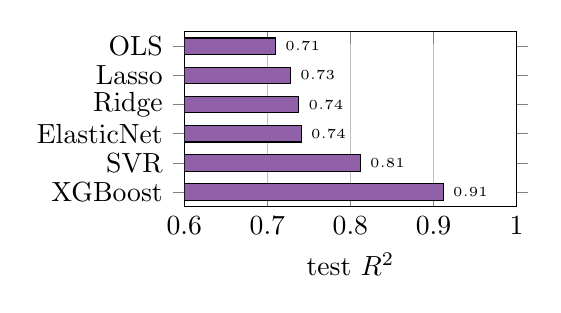
\begin{tikzpicture}\begin{axis}[xbar,width=5.8cm,height=3.8cm,symbolic y coords={XGBoost,SVR,ElasticNet,Ridge,Lasso,OLS},ytick=data,xmin=0.6,xmax=1,bar width=6pt,nodes near coords,nodes near coords style={font=\fontsize{5.5}{6}\selectfont},xlabel={test $R^2$},xmajorgrids]
\addplot[fill=AccentCol!75]coordinates{(0.912,XGBoost)(0.812,SVR)(0.741,ElasticNet)(0.738,Ridge)(0.728,Lasso)(0.710,OLS)};
\end{axis}\end{tikzpicture}}
\begin{cbox}[ISSAnavy]{Which penalty?}\scriptsize \textbf{Ridge:} default for collinear features, keep all. \textbf{Lasso:} when many features are irrelevant. \textbf{Elastic Net:} unknown structure --- the recommended default; two hyper-parameters.\end{cbox}
\end{columns}
\end{frame}

\sect{4. SVR \& Boosting}
\begin{frame}{Support Vector Regression --- Fitting Within a Tube: No Penalty for Small Errors}
\begin{columns}[T]
\column{0.50\textwidth}
\figc{3.2cm}{\begin{tikzpicture}\begin{axis}[width=6.8cm,height=3.9cm,xlabel={$x$},ylabel={$y$},domain=0:6,samples=60,ticks=none,ymin=-0.8,ymax=3.4]
\addplot[AccentCol,thick]{1.6+sin(deg(x))*1.1};\addplot[AccentCol!60,dashed]{1.6+sin(deg(x))*1.1+0.4};\addplot[AccentCol!60,dashed]{1.6+sin(deg(x))*1.1-0.4};
\addplot[name path=up,draw=none]{1.6+sin(deg(x))*1.1+0.4};\addplot[name path=lo,draw=none]{1.6+sin(deg(x))*1.1-0.4};\addplot[AccentCol!15]fill between[of=up and lo];
\addplot[only marks,mark=*,mark size=1.1pt,ISSAblue]coordinates{(0.4,1.9)(1.0,2.6)(1.8,2.5)(2.4,1.9)(3.0,1.6)(3.6,0.9)(4.2,0.4)(5.0,0.6)(5.6,1.5)};
\addplot[only marks,mark=*,mark size=1.4pt,ISSAred]coordinates{(1.4,3.1)(4.6,-0.4)(2.9,2.4)};
\node[font=\tiny,ISSAred,anchor=west]at(axis cs:1.5,3.2){outside tube: penalised ($\xi$)};\node[font=\tiny,AccentCol,anchor=south]at(axis cs:5.0,2.1){$\varepsilon$-tube};
\end{axis}\end{tikzpicture}}
\begin{fbx}{$\varepsilon$-insensitive loss and primal}\[L_\varepsilon(y,\hat y)=\max\big(0,|y-\hat y|-\varepsilon\big)\]\[\min\tfrac12\|w\|^{2}+C\sum_i(\xi_i+\xi_i^{*})\]\end{fbx}
\column{0.48\textwidth}
\begin{tl}\item Constraints: $y_i-w^{\top}x_i-b\le\varepsilon+\xi_i$ (upper), $w^{\top}x_i+b-y_i\le\varepsilon+\xi_i^{*}$ (lower), $\xi,\xi^{*}\ge0$\item \textbf{$C$:} tolerance for errors OUTSIDE the tube; large $C$ = tight fit (may overfit)\item \textbf{$\varepsilon$:} half-width of the tube; larger $\varepsilon$ = more points inside = sparser model\item Prediction $\hat y=\sum_i(\alpha_i-\alpha_i^{*})K(x_i,x)+b$ (RBF kernel for Case A)\end{tl}
\begin{rbox}\scriptsize\textbf{Case A grid search:} $C=50$, $\varepsilon=0.5$, $\gamma=0.05$: test $R^2=0.812$, RMSE 3.24 h; \textbf{1,842 support vectors (42.4\%} of training data).\end{rbox}
\end{columns}
\end{frame}

\begin{frame}{Why SVR in Defence Regression --- Benefits and Trade-off}
\begin{columns}[T]
\column{0.50\textwidth}
\begin{cbox}[ISSAgrn]{Benefit 1: robust to outliers}\scriptsize Training data has extreme battles (2-hour ops to 48-hour sieges). With $\varepsilon=0.5$, prediction errors under 30 min are IGNORED --- the model focuses on getting the large errors right.\end{cbox}
\begin{cbox}[ISSAgrn]{Benefit 2: non-parametric kernel mapping}\scriptsize RBF captures non-linear terrain--duration relationships linear methods miss: mountain terrain + rain is a \emph{multiplicative} effect, not additive.\end{cbox}
\begin{cbox}[ISSAgrn]{Benefit 3: sparse model via support vectors}\scriptsize Inference $\propto$ \#SVs $\times$ kernel cost, independent of $N$ once the SVs are found.\end{cbox}
\column{0.48\textwidth}
\subhead{Training time vs sample size}
\figc{2.9cm}{\begin{tikzpicture}\begin{axis}[width=6.4cm,height=3.5cm,xlabel={training samples $N$ (thousands)},ylabel={time (s)},xmin=0,xmax=45,ymin=0,ymax=560,ymajorgrids]
\addplot[ISSAred,thick,mark=*,domain=0:42,samples=2]coordinates{(0,0)(4.34,4.8)(40,480)};
\node[font=\tiny,anchor=south east]at(axis cs:4.34,4.8){4,340: 4.8 s};\node[font=\tiny,ISSAred,anchor=south east]at(axis cs:40,480){40,000: $\sim$480 s (too slow!)};
\end{axis}\end{tikzpicture}}
\sm{Straight-line extrapolation from the reported 4,340 $\to$ 40,000 sample figures; kernel SVR is $O(N^2)$--$O(N^3)$, so real growth can be worse.}
\begin{wbox}\scriptsize\textbf{Trade-off:} kernel SVR training is $O(N^2)$ to $O(N^3)$: 4,340 samples $\to$ 4.8 s is fine; 40,000 samples would take $\sim$480 s. Use \textbf{XGBoost} for large datasets.\end{wbox}
\end{columns}
\end{frame}

\begin{frame}{Gradient Boosting for Regression --- XGBRegressor: Sequential Residual Learning}
\begin{columns}[T]
\column{0.52\textwidth}
\figc{2.1cm}{\begin{tikzpicture}\node[nd](f0)at(0,0){$F_0=\bar y$};\foreach \i/\x in {1/2.1,2/4.2,3/6.3}{\node[ndG,minimum width=1.5cm](t\i)at(\x,0){tree $T_\i$\\\sm{fits residuals $r_{i}$}};}\node[ndA](f)at(8.6,0){$F_M=\bar y+\eta\sum T_m$};\draw[arr](f0)--(t1);\draw[arr](t1)--(t2);\draw[arr](t2)--(t3);\draw[arr](t3)--(f);\node[lab]at(4.3,-0.85){$r_{im}=y_i-F_{m-1}(x_i)$: what the model got wrong; trees predict residuals, NOT the target};\end{tikzpicture}}
\begin{fbx}{Update and XGBoost objective}\[F_m(x)=F_{m-1}(x)+\eta\,T_m(x)\ (\eta=0.05,\ \text{depth }5)\]\[\mathcal{L}=\sum_i(y_i-\hat y_i)^{2}+\sum_m\Omega(T_m),\ \ \Omega(T)=\gamma|\text{leaves}|+\tfrac12\lambda\|w\|^{2}\]\end{fbx}
\sm{Second-order Taylor expansion is used for speed. Hyper-parameters (5-fold CV): $M=400$, $\eta=0.05$, depth 5, subsample 0.8, colsample 0.8, $\alpha=0.1$, $\lambda=1.0$.}
\column{0.46\textwidth}
\figc{2.4cm}{\begin{tikzpicture}\begin{axis}[width=6.2cm,height=3.2cm,xmode=log,xlabel={number of trees $M$},ylabel={val. RMSE (h)},xmin=8,xmax=1500,ymin=1.5,ymax=7.2,ymajorgrids]
\addplot[AccentCol,thick,mark=*,mark size=1.2pt]coordinates{(10,6.81)(50,4.23)(100,3.42)(200,2.68)(400,2.11)(800,2.19)(1200,2.34)};
\node[font=\tiny,ISSAgrn,anchor=south west]at(axis cs:300,2.4){optimum $M{=}400$};\node[font=\tiny,ISSAred,anchor=south]at(axis cs:1100,2.55){overfit starts};
\end{axis}\end{tikzpicture}}
\figc{2.0cm}{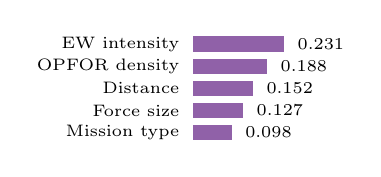
\begin{tikzpicture}[x=5cm,y=0.28cm]\foreach \i/\lbl/\v in {0/EW intensity/0.231,1/OPFOR density/0.188,2/Distance/0.152,3/Force size/0.127,4/Mission type/0.098}{\fill[AccentCol!75](0,-\i-0.35)rectangle(\v,-\i+0.35);\node[font=\fontsize{5.8}{6}\selectfont,anchor=east]at(-0.01,-\i){\lbl};\node[font=\fontsize{5.8}{6}\selectfont,anchor=west]at(\v+0.01,-\i){\v};}\end{tikzpicture}}
\begin{rbox}\scriptsize\textbf{Final test:} $R^2=0.912$, RMSE 2.06 h, MAE 1.54 h; importances consistent with the OLS coefficients.\end{rbox}
\end{columns}
\end{frame}

\sect{5. Metrics \& Uncertainty}
\begin{frame}{Regression Metrics --- What They Measure and When They Mislead}
\begin{columns}[T]
\column{0.50\textwidth}
\begin{fbx}{The four core metrics}\[\text{MSE}=\tfrac1N\sum(y_i-\hat y_i)^{2},\quad\text{RMSE}=\sqrt{\text{MSE}}\]\[\text{MAE}=\tfrac1N\sum|y_i-\hat y_i|,\quad\text{MAPE}=\tfrac{100}{N}\sum\tfrac{|y_i-\hat y_i|}{|y_i|}\]\[R^{2}=1-\tfrac{SS_{\text{res}}}{SS_{\text{tot}}},\quad \text{Adj.}R^{2}=1-(1-R^{2})\tfrac{N-1}{N-d-1}\]\end{fbx}
\figc{2.0cm}{\bars{3}{1.4}{1.9}{RMSE 2.06 h/2.06/ISSAred,MAE 1.54 h/1.54/ISSAblue,MAPE 8.3\%/0.83/ISSAamb}}
\sm{XGBoost, Case A. RMSE $>$ MAE confirms outlier battles exist. $R^2=0.912$: the model explains 91.2\% of variance in mission duration. (MAPE bar scaled $\times0.1$.)}
\column{0.48\textwidth}
\begin{wbox}\scriptsize\textbf{Metric traps in defence regression}\begin{tl}\item \textbf{Trap 1:} high train $R^2$, low test $R^2$ (0.98 vs 0.71) = overfitting; report both (OLS: 0.738 vs 0.710)\item \textbf{Trap 2:} RMSE hides \emph{directional bias}: missions taking LONGER than predicted is critical for logistics; report signed mean bias $\sum(y_i-\hat y_i)/N$\item \textbf{Trap 3:} $R^2$ can be \emph{negative} if the model is worse than predicting the mean ($SS_{\text{res}}>SS_{\text{tot}}$)\item \textbf{Trap 4:} time-series exercise data inflate $R^2$ via autocorrelation $\Rightarrow$ use an out-of-time test\item \textbf{Trap 5:} MAPE is undefined when $y_i=0$; use sMAPE or RMSE\end{tl}\end{wbox}
\end{columns}
\end{frame}

\begin{frame}{Prediction Uncertainty --- Knowing When Your Model Doesn't Know}
\begin{columns}[T]
\column{0.50\textwidth}
\figc{3.1cm}{\begin{tikzpicture}\begin{axis}[width=6.8cm,height=3.7cm,xlabel={scenario complexity (feature space)},ylabel={mission duration (h)},domain=0:10,samples=40,ticks=none,ymin=0,ymax=40]
\addplot[name path=up,draw=none]{8+2*x+0.5+0.35*x^1.6};\addplot[name path=lo,draw=none]{8+2*x-0.5-0.35*x^1.6};\addplot[AccentCol!20]fill between[of=up and lo];
\addplot[AccentCol,thick]{8+2*x};
\addplot[only marks,mark=*,mark size=1pt,ISSAblue]coordinates{(0.5,9.5)(1,9.7)(1.6,11.9)(2.1,11.8)(2.7,14.1)(3.2,14.0)(3.8,15.9)(4.3,16.9)(5,18.5)(5.6,19.2)(6.2,20.9)(6.8,21.5)(7.5,24)(8.2,23)};
\node[font=\tiny,anchor=south]at(axis cs:7.8,34){wide: sparse region};\node[font=\tiny,anchor=north]at(axis cs:1.5,7){narrow: dense data};
\end{axis}\end{tikzpicture}}
\begin{fbx}{OLS prediction interval}\[\hat y_{\text{new}}\pm t_{N-d-1,\alpha/2}\,\hat s\sqrt{1+x^{\top}(X^{\top}X)^{-1}x}\]\end{fbx}
\column{0.48\textwidth}
\begin{cbox}[ISSAnavy]{Why it matters}\scriptsize ``Mission takes 18.4 h'' is operationally incomplete. The commander needs ``$\pm$ what?'', the 90\% upper bound, ``should I plan for 22 h?''.\end{cbox}
\begin{tl}\item \textbf{Aleatoric} (irreducible): random enemy behaviour, weather; not reduced by more data\item \textbf{Epistemic} (model ignorance): sparse training regions; reducible with more data\end{tl}
\begin{cbox}[ISSAgrn]{Practical intervals}\scriptsize \textbf{RF/XGBoost:} $\hat y\pm1.645\,\sigma_{\text{pred}}$ from variance over $B=500$ trees: average width $\pm3.8$ h. \textbf{Bayesian ridge} ($w\sim\mathcal{N}(0,\tfrac{\sigma^2}{\lambda}I)$, posterior $\mathcal{N}(w_{\text{Ridge}},\sigma^2(X^{\top}X+\lambda I)^{-1})$): avg 95\% CI $\pm6.1$ h; 90\% coverage \textbf{89.4\%} (well calibrated); in sparse regions CI widens to $\pm12+$ h.\end{cbox}
\begin{rbox}\scriptsize\textbf{Defence value:} ``18.4 h but $\pm12$ h for this mountain-jungle mission'' beats blindly reporting 18.4 h with false precision.\end{rbox}
\end{columns}
\end{frame}

\sect{5b. Casualty \& Force Regression}
\begin{frame}{Casualty Estimates Are Counts --- Poisson Regression for Planning}
\begin{columns}[T]
\column{0.50\textwidth}
\begin{fbx}{Poisson regression (a generalised linear model)}\[Y\sim\text{Poisson}(\mu),\qquad\ln\mu=\beta_0+\beta_1x_1+\cdots\]\end{fbx}
\begin{tl}\scriptsize\item log link keeps $\mu>0$; effects are \textbf{multiplicative}: rate ratio $e^{\beta_j}$
\item \textbf{offset} $\ln(\text{exposure})$ for unequal unit-days or strengths
\item OLS would predict negative counts and assume constant variance
\end{tl}
\begin{cbox}{Worked example: casualties per company-day}\scriptsize Fitted on simulated engagements: $\ln\mu=0.5+0.25\,x$, $x$ = enemy artillery battalions in range.\\ Rate ratio $e^{0.25}=\mathbf{1.28}$: +28\% per battalion.\\ $x=0$: $\mu=1.65$;\quad $x=2$: $\mu=2.72$;\quad $x=4$: $\mu=\mathbf{4.48}$\end{cbox}
\begin{wbox}\scriptsize\textbf{Over-dispersion:} real casualty data have catastrophic tails (variance $>$ mean). Check deviance/df; use the \textbf{negative binomial} model for honest, wider intervals.\end{wbox}
\column{0.48\textwidth}
\subhead{Plan against the tail, not the mean ($x=4$)}
\figc{3.3cm}{\begin{tikzpicture}\begin{axis}[ybar,bar width=6pt,width=6.4cm,height=4.2cm,xmin=-0.7,xmax=12.7,ymin=0,ymax=0.21,xlabel={casualties per company-day},ylabel={probability},xtick={0,2,...,12},font=\tiny,ymajorgrids,bar shift=0pt,yticklabel style={/pgf/number format/fixed,/pgf/number format/precision=2},scaled y ticks=false]
\addplot[fill=AccentCol!70,draw=none]coordinates{(0,0.011)(1,0.051)(2,0.114)(3,0.170)(4,0.190)(5,0.170)(6,0.127)(7,0.082)};
\addplot[fill=ISSAred!75,draw=none]coordinates{(8,0.046)(9,0.023)(10,0.010)(11,0.004)(12,0.002)};
\draw[dashed,ISSAnavy](axis cs:4.48,0)--(axis cs:4.48,0.205);\node[font=\tiny,anchor=west,fill=white,inner sep=1pt]at(axis cs:7.2,0.17){mean $\mu=4.48$};
\end{axis}\end{tikzpicture}}
\begin{ibox}\scriptsize $P(\ge8)=\mathbf{8.5\%}$; 95th percentile $=8$. Medical and evacuation capacity should be sized for $\approx8$, not 4.5.\end{ibox}
\begin{rbox}\scriptsize Casualty estimates are \textbf{planning inputs}, not forecasts of fact: report ranges with stated assumptions; the uncertainty must reach the commander.\end{rbox}
\end{columns}
\end{frame}

\begin{frame}{Force Effectiveness --- Estimating Lanchester Coefficients by Regression}
\begin{columns}[T]
\column{0.50\textwidth}
\begin{fbx}{Lanchester square law (aimed fire)}\[\frac{dB}{dt}=-r\,R,\qquad\frac{dR}{dt}=-b\,B\]\vspace{-6pt}\[\Rightarrow\;b(B_0^2-B^2)=r(R_0^2-R^2)\]\end{fbx}
\begin{cbox}{Worked example: Red's kill rate from a simulation}\scriptsize Red strength $R$: 100, 80, 60 tanks; Blue losses $\Delta B$: 5.1, 4.0, 3.1 per hour.\\ Regression through the origin: $\hat r=\dfrac{\sum R\,\Delta B}{\sum R^2}=\dfrac{1{,}016}{20{,}000}=\mathbf{0.0508}$ per Red tank per hour. Fitted 5.08, 4.06, 3.05 --- consistent with the square law.\end{cbox}
\begin{tl}\scriptsize\item \textbf{Which law?} Fit $\ln\Delta B=\ln c+p\ln R+q\ln B$: square law $p=1,q=0$; linear law $p=1,q=1$. Historical fits fall in between.
\item Modern models regress effectiveness on terrain, weather, morale, EW: $R^2$ 0.61 $\to$ 0.87 (L1 example).\end{tl}
\column{0.48\textwidth}
\figc{2.9cm}{\begin{tikzpicture}\begin{axis}[width=6.2cm,height=4.0cm,xmin=0,xmax=110,ymin=0,ymax=6,xlabel={Red strength $R$},ylabel={Blue losses / h},grid=major,font=\tiny]
\addplot[AccentCol,thick,domain=0:110]{0.0508*x};
\addplot[only marks,mark=*,ISSAnavy]coordinates{(100,5.1)(80,4.0)(60,3.1)};
\node[font=\tiny,anchor=north west]at(axis cs:5,5.5){$\Delta B=0.0508\,R$};
\end{axis}\end{tikzpicture}}
\begin{rbox}\scriptsize\textbf{Force-ratio planning:} Blue prevails if $bB_0^2>rR_0^2$, i.e.\ $\dfrac{B_0}{R_0}>\sqrt{r/b}$. If Red's kill rate is \textbf{4$\times$} Blue's, Blue needs \textbf{2$\times$} Red's numbers, not 4$\times$.\end{rbox}
\begin{wbox}\scriptsize $\sqrt{r/b}$ combines two uncertain estimates non-linearly: bootstrap the engagements and report an interval before using it in planning.\end{wbox}
\end{columns}
\end{frame}

\sect{6. Kalman Filter}
\begin{frame}{Kalman Filter --- Predict, Measure, Fuse: Recursively \& Optimally}
\begin{columns}[T]
\column{0.50\textwidth}
\figc{3.0cm}{\begin{tikzpicture}
\node[ndA,minimum width=2.4cm,minimum height=1.0cm](p)at(0,0){\textbf{PREDICT}\\\sm{$\hat x^{-}=F\hat x^{+}_{\text{prev}}$}\\\sm{$P^{-}=FP^{+}F^{\top}+Q$}};
\node[ndG,minimum width=2.4cm,minimum height=1.0cm](u)at(4.2,0){\textbf{UPDATE}\\\sm{$K,\ \hat x^{+},\ P^{+}$}};
\node[ndY](z)at(4.2,1.6){sensor measurement $z_k$};\node[nds](o)at(6.6,0){track estimate $\hat x_k^{+}$};\draw[arr](u)--(o);
\draw[bigarr](p)--node[above,lab]{prior}(u);\draw[bigarr](u.south)--++(0,-0.75)-|(p.south);\node[lab]at(2.1,-1.0){next step $k\to k{+}1$};\draw[arr](z)--(u);
\end{tikzpicture}}
\begin{fbx}{State-space model}\[x_k=Fx_{k-1}+Bu_k+w_k,\ \ w_k\sim\mathcal{N}(0,Q)\]\[z_k=Hx_k+v_k,\ \ v_k\sim\mathcal{N}(0,R)\]\end{fbx}
\column{0.48\textwidth}
\begin{fbx}{Update step (innovation $\nu_k=z_k-H\hat x_k^{-}$)}\[K_k=P_k^{-}H^{\top}\big(HP_k^{-}H^{\top}+R\big)^{-1}\]\[\hat x_k^{+}=\hat x_k^{-}+K_k\nu_k,\quad P_k^{+}=(I-K_kH)P_k^{-}\]\end{fbx}
\begin{tl}\item $x_k$: state (position, velocity, heading); $F$: transition; $Bu_k$: known manoeuvres; $w_k$: model error\item $z_k$: sensor measurement (radar return); $H$: maps state to observation; $v_k$: sensor noise\end{tl}
\begin{cbox}[ISSAnavy]{3-sensor Case B setup}\scriptsize State $x=[X,Y,\dot X,\dot Y]^{\top}$ for each of 5 targets. \textbf{Radar} $R=\text{diag}(50^2,0.5^2,10^2)$ (range $\pm$50 m, bearing $\pm0.5^\circ$, speed $\pm$10 km/h). \textbf{IR} $R=\text{diag}(0.8^2,1.2^2)$ (angle-only). \textbf{ELINT} $R=\text{diag}(0.1^2,0.2^2,5^2)$ (freq, PRF, bearing $\pm5^\circ$).\end{cbox}
\end{columns}
\end{frame}

\begin{frame}{Kalman Gain Intuition --- How Much to Trust the Measurement}
\begin{columns}[T]
\column{0.50\textwidth}
\figc{3.3cm}{\begin{tikzpicture}\begin{axis}[width=6.6cm,height=3.8cm,xmode=log,xlabel={measurement noise / prediction uncertainty ($R/P^{-}$)},ylabel={scalar gain $K=\frac{P^{-}}{P^{-}+R}$},xmin=0.01,xmax=100,ymin=0,ymax=1,domain=0.01:100,samples=60,ymajorgrids]
\addplot[AccentCol,thick]{1/(1+x)};
\node[font=\tiny,ISSAgrn,anchor=south west]at(axis cs:0.012,0.9){$R\ll P^{-}$: trust the MEASUREMENT};\node[font=\tiny,ISSAred,anchor=south east]at(axis cs:95,0.1){$R\gg P^{-}$: trust the PREDICTION};\fill[ISSAamb](axis cs:1,0.5)circle(1.5pt);\node[font=\tiny,anchor=south west]at(axis cs:1.1,0.5){equal trust};
\end{axis}\end{tikzpicture}}
\begin{tl}\item $K_k\to0$ when $R\gg P^{-}H^{\top}H$: sensor noise exceeds prediction uncertainty $\Rightarrow$ trust the \textbf{prediction}\item $K_k\to H^{-1}$ when $R\ll P^{-}H^{\top}H$: trust the \textbf{measurement}, override the prediction\end{tl}
\column{0.48\textwidth}
\begin{cbox}[ISSAgrn]{Illustrative 1-D worked update (not exercise data)}\scriptsize Prior $\hat x^{-}=100$ km, $P^{-}=4$; radar reads $z=104$ km with $R=1$.\\ $K=\dfrac{4}{4+1}=0.8$ \quad $\hat x^{+}=100+0.8(104-100)=\mathbf{103.2}$ km \quad $P^{+}=(1-0.8)(4)=\mathbf{0.8}$.\\ A precise radar pulls the estimate 80\% of the way toward the measurement and cuts the variance five-fold.\end{cbox}
\figc{1.9cm}{\begin{tikzpicture}\begin{axis}[width=6.2cm,height=2.4cm,xlabel={position (km)},ticks=none,domain=92:112,samples=60,ymin=0,legend pos=north west,legend columns=3]
\addplot[ISSAblue,thick]{exp(-(x-100)^2/(2*4))/sqrt(2*pi*4)};\addlegendentry{prior}
\addplot[ISSAred,thick]{exp(-(x-104)^2/(2*1))/sqrt(2*pi*1)};\addlegendentry{meas.}
\addplot[ISSAgrn,thick]{exp(-(x-103.2)^2/(2*0.8))/sqrt(2*pi*0.8)};\addlegendentry{fused}
\end{axis}\end{tikzpicture}}
\sm{Fused estimate is narrower than either input: fusion always reduces uncertainty.}
\end{columns}
\end{frame}

\sect{7. Sensor Fusion}
\begin{frame}{Multi-Sensor Fusion --- Architecture Choices: Early, Late \& Hybrid}
\figc{2.4cm}{\begin{tikzpicture}
\begin{scope}\node[font=\scriptsize\bfseries,AccentCol]at(1.6,2.1){EARLY (feature-level)};\foreach \i/\n in {0/Radar,1/IR,2/ELINT}{\node[nds,minimum width=1.0cm](a\i)at(0,1.4-\i*0.7){\n};}\node[ndN,minimum width=1.2cm,minimum height=1.6cm](m)at(1.9,0.7){single\\model};\node[ndG](o)at(3.4,0.7){track};\foreach \i in {0,1,2}{\draw[arr](a\i)--(m);}\draw[arr](m)--(o);\end{scope}
\begin{scope}[xshift=4.9cm]\node[font=\scriptsize\bfseries,AccentCol]at(1.9,2.1){LATE (decision-level)};\foreach \i/\n in {0/Radar,1/IR,2/ELINT}{\node[nds,minimum width=1.0cm](b\i)at(0,1.4-\i*0.7){\n};\node[ndN,minimum width=0.9cm](c\i)at(1.5,1.4-\i*0.7){model};\draw[arr](b\i)--(c\i);}\node[ndA,minimum width=0.9cm,minimum height=1.6cm](v)at(3.0,0.7){vote};\foreach \i in {0,1,2}{\draw[arr](c\i)--(v);}\node[ndG](o2)at(4.2,0.7){track};\draw[arr](v)--(o2);\end{scope}
\begin{scope}[xshift=10.3cm]\node[font=\scriptsize\bfseries,AccentCol]at(2.0,2.1){HYBRID (ML-enhanced KF)};\node[nds,minimum width=1.0cm](d)at(0,0.7){3 sensors};\node[ndN,minimum width=1.2cm,minimum height=1.0cm](kf)at(1.7,0.7){Kalman\\filter};\node[ndA,minimum width=1.1cm](rf)at(3.3,1.4){RF bias\\corrector};\node[ndG](o3)at(4.5,0.7){track};\draw[arr](d)--(kf);\draw[arr](kf)--(o3);\draw[arr](kf.north)--(rf.west);\draw[arr](rf.south)--(o3.north);\node[lab]at(3.2,0.0){$\hat x_{KF}+\delta x$};\end{scope}
\end{tikzpicture}}
\begin{columns}[T]
\column{0.33\textwidth}
\begin{cbox}[ISSAred]{Early fusion: 91.4\%}\scriptsize $\checkmark$ learns cross-sensor correlations; one model. $\times$ fails with missing data; sensitive to different sampling rates; high-dim input needs more data.\end{cbox}
\column{0.33\textwidth}
\begin{cbox}[ISSAamb]{Late fusion: 89.7\%}\scriptsize $\checkmark$ robust to sensor failure (omit); different model per sensor; easy to add/remove sensors. $\times$ loses cross-sensor correlations; each sub-model needs full labels.\end{cbox}
\column{0.33\textwidth}
\begin{cbox}[ISSAgrn]{Hybrid: 96.2\% --- best}\scriptsize KF handles timing \& physics; ML corrects systematic bias in KF residuals: $\delta x=g(\nu_k,\text{feat}_k;\theta)$, $\hat x_{\text{final}}=\hat x_{KF}+\delta x$. Physics-grounded, interpretable, handles rare events.\end{cbox}
\end{columns}
\begin{ibox}\scriptsize\textbf{Recommended for IADS fusion: hybrid (ML-enhanced Kalman).} A standard KF assumes linear dynamics and Gaussian noise --- both violated in combat (evasive manoeuvres, jamming spikes); ML corrects both. Long pedigree in missile guidance.\end{ibox}
\end{frame}

\begin{frame}{Case Study B --- 3-Sensor Fusion Results (5 Targets, 10 Runs)}
\begin{columns}[T]
\column{0.52\textwidth}
\subhead{Target-assignment accuracy by method (\%)}
\figc{3.9cm}{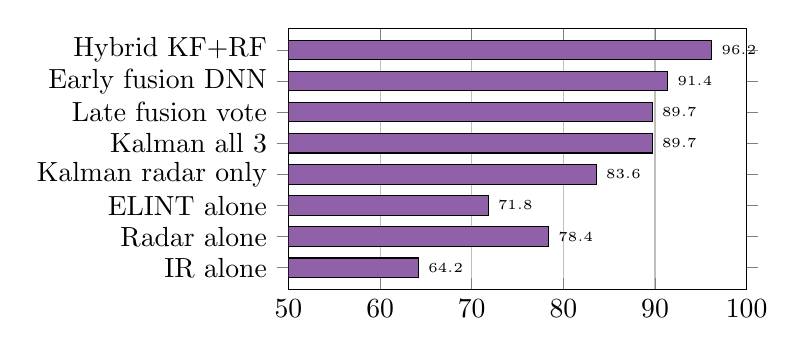
\begin{tikzpicture}\begin{axis}[xbar,width=7.4cm,height=4.9cm,symbolic y coords={Hybrid KF+RF,Early fusion DNN,Late fusion vote,Kalman all 3,Kalman radar only,ELINT alone,Radar alone,IR alone},ytick=data,xmin=50,xmax=100,bar width=7pt,nodes near coords,nodes near coords style={font=\fontsize{5.5}{6}\selectfont},xmajorgrids,y dir=reverse]
\addplot[fill=AccentCol!75]coordinates{(96.2,Hybrid KF+RF)(91.4,Early fusion DNN)(89.7,Late fusion vote)(89.7,Kalman all 3)(83.6,Kalman radar only)(71.8,ELINT alone)(78.4,Radar alone)(64.2,IR alone)};
\end{axis}\end{tikzpicture}}
\column{0.46\textwidth}
\subhead{Robustness: IR missing 20\% of the time (cloud)}
\figc{2.5cm}{\begin{tikzpicture}\begin{axis}[ybar,width=6.4cm,height=3.2cm,symbolic x coords={Kalman (3),Early DNN,Hybrid KF+RF},xtick=data,ymin=60,ymax=100,bar width=11pt,enlarge x limits=0.25,legend style={at={(0.5,1.03)},anchor=south,legend columns=2},nodes near coords,nodes near coords style={font=\fontsize{5.5}{6}\selectfont},ymajorgrids]
\addplot[fill=ISSAblue!60]coordinates{(Kalman (3),89.7)(Early DNN,91.4)(Hybrid KF+RF,96.2)};\addlegendentry{no gap}
\addplot[fill=ISSAred!65]coordinates{(Kalman (3),82.1)(Early DNN,74.8)(Hybrid KF+RF,94.8)};\addlegendentry{20\% IR gap}
\end{axis}\end{tikzpicture}}
\figc{1.8cm}{\scriptsize\begin{tabular}{lc}\toprule Method&Latency\\\midrule Radar alone&0.3 ms\\Kalman (all 3)&1.2 ms\\Early DNN&3.8 ms\\Late vote&4.1 ms\\\textbf{Hybrid KF+RF}&\textbf{2.3 ms}\\\bottomrule\end{tabular}}
\begin{rbox}\scriptsize The hybrid loses only 1.4 points under the IR gap; the early-fusion DNN loses 16.6.\end{rbox}
\end{columns}
\end{frame}

\begin{frame}{How the Hybrid Model Works --- ML Corrects the Kalman Residuals}
\figc{2.2cm}{\begin{tikzpicture}\tikzset{S/.style={ndA,text width=2.7cm,minimum height=1.3cm}}
\node[S](a)at(0,0){\textbf{1 Kalman update}\\run the standard 3-sensor KF: $\hat x_{KF},P_{KF},\nu_k$ per target};\node[S](b)at(3.3,0){\textbf{2 Residual features}\\$f_k$: innovation $\nu_k$, $\|\nu_k\|^2$, $S_k$, $\Delta t_k$, sensor availability};\node[S](c)at(6.6,0){\textbf{3 RF bias corrector}\\$\delta x_k=\text{RF}(f_k)$, trained on true-minus-KF error pairs};\node[S,fill=ISSAgrn!15,draw=ISSAgrn](d)at(9.9,0){\textbf{4 Apply}\\$\hat x_{\text{final}}=\hat x_{KF}+\delta x_k$};
\foreach \u/\v in {a/b,b/c,c/d}{\draw[bigarr](\u)--(\v);}
\end{tikzpicture}}
\begin{columns}[T]
\column{0.50\textwidth}
\begin{cbox}[ISSAnavy]{Why residuals as features?}\scriptsize The innovation $\nu_k=z_k-H\hat x_k^{-}$ encodes how much reality differs from the KF prediction, sensor-specific bias patterns, and manoeuvre signatures the KF missed. $S_k=HP_k^{-}H^{\top}+R$ is the innovation covariance; $\Delta t_k$ = time since each sensor last updated. The RF learns the systematic \emph{non-Gaussian} patterns in $\nu$.\end{cbox}
\column{0.48\textwidth}
\figc{2.7cm}{\begin{tikzpicture}\begin{axis}[width=6.2cm,height=3.3cm,xlabel={time step},ylabel={position error (m)},ymajorgrids,domain=0:20,samples=40,legend pos=north west]
\addplot[ISSAred,thick]{35+25*sin(deg(x*0.5))+8*x/4};\addlegendentry{KF (manoeuvre bias)}
\addplot[ISSAgrn,thick]{12+6*sin(deg(x*0.5))+1.5*x/4};\addlegendentry{KF + RF correction}
\end{axis}\end{tikzpicture}}
\sm{Schematic: RF removes the systematic manoeuvre-correlated component of the KF error.}
\end{columns}
\end{frame}

\begin{frame}{Handling Missing Data in Sensor Fusion --- Dropouts and Out-of-Sequence Measurements}
\begin{columns}[T]
\column{0.50\textwidth}
\begin{cbox}[ISSAred]{Why sensors go missing}\scriptsize \textbf{Radar:} terrain dead zones, jamming (30--80\% loss), ducting. \textbf{IR:} cloud, precipitation, clutter, vibration (15--40\% degradation). \textbf{ELINT:} enemy EMCON, LPI emissions. In Case B, IR is blocked 20\% of the time.\end{cbox}
\subhead{Accuracy impact of each imputation strategy}
\figc{2.3cm}{\bars{3}{1.5}{2.0}{Mean or median imputation/2.1/ISSAred,Last obs. carried fwd/1.4/ISSAamb,KF prediction as imputation/0.8/ISSAblue,ML cross-sensor imputation/0.3/ISSAgrn}}
\sm{Accuracy loss in points (lower is better). Best: ML cross-sensor imputation (RF predicts IR from radar + ELINT).}
\column{0.48\textwidth}
\subhead{Out-of-sequence measurements (OOSM)}
\figc{2.0cm}{\begin{tikzpicture}\draw[->](0,0)--(7,0)node[right,font=\tiny]{time};\foreach \x/\l in {1/{$z_1$},2.5/{$z_2$ (taken $t_2$)},4.5/{$z_3$}}{\fill[AccentCol](\x,0)circle(0.08);\node[font=\tiny,anchor=south]at(\x,0.1){\l};}\draw[ISSAred,thick,->](5.5,0.7)--(2.5,0.7)node[midway,above,font=\tiny]{arrives late, after $z_3$};\draw[ISSAgrn,thick,->](2.5,-0.6)--(5.5,-0.6)node[midway,below,font=\tiny]{roll back, apply, re-propagate};\end{tikzpicture}}
\sm{Naive KF processes in arrival order: error. The radar update arrives 0.3 s after it was taken; retro-correct by rolling back to the measurement time, applying it, then re-propagating.}
\begin{wbox}\scriptsize\textbf{Data pitfall:} naive imputation can CORRUPT fusion by introducing \emph{false precision} --- a filled-in IR bearing looks as certain as a real one (the KF assigns it the same $R$). Track imputation flags and \textbf{inflate $R$} for imputed measurements.\end{wbox}
\end{columns}
\end{frame}

\begin{frame}{Extended and Unscented Kalman Filters --- Non-linear Tracking}
\begin{columns}[T]
\column{0.52\textwidth}
\figc{3.2cm}{\begin{tikzpicture}\begin{axis}[width=6.4cm,height=3.8cm,xlabel={state $x$},ylabel={$f(x)$},domain=0:4,samples=50,ticks=none]
\addplot[AccentCol,thick]{1+1.2*x-0.35*x^2+0.3*sin(deg(2*x))};
\addplot[ISSAred,dashed,thick,domain=0.4:3.2]{1.55+0.95*(x-1.5)};
\node[font=\tiny,ISSAred,anchor=south west]at(axis cs:2.6,3.4){EKF: tangent (Jacobian)};
\fill[ISSAgrn](axis cs:1.0,0.0)circle(1.4pt);\fill[ISSAgrn](axis cs:1.5,0.0)circle(1.4pt);\fill[ISSAgrn](axis cs:2.0,0.0)circle(1.4pt);\node[font=\tiny,ISSAgrn,anchor=north]at(axis cs:1.5,0.1){UKF sigma points};
\end{axis}\end{tikzpicture}}
\column{0.46\textwidth}
\begin{cbox}[ISSAred]{Extended Kalman Filter (EKF)}\scriptsize Standard KF: linear dynamics only. EKF linearises $f(x)$ around the current estimate: $F_k=\partial f/\partial x\big|_{x=\hat x_{k-1}}$ (the Jacobian) and replaces $F$ at every step. Applicable to aircraft evasive manoeuvres; truncation error from linearisation.\end{cbox}
\begin{cbox}[ISSAgrn]{Unscented Kalman Filter (UKF)}\scriptsize Propagates a small set of carefully chosen \textbf{sigma points} through the non-linear function exactly --- no Jacobian. Better than EKF for strongly non-linear dynamics: hypersonic target tracking, UAV swarms.\end{cbox}
\begin{ibox}\scriptsize Combat violates both KF assumptions: dynamics are non-linear (EKF/UKF) and noise is non-Gaussian (ML bias correction).\end{ibox}
\end{columns}
\end{frame}

\sect{8. Unified Results}
\begin{frame}{Lecture 3 --- Unified Results: Regression \& Sensor Fusion Side by Side}
\begin{columns}[T]
\column{0.52\textwidth}
\subhead{Case A: mission-duration regression ($N=6{,}200$, 18 features)}
\figc{3.0cm}{\scriptsize\renewcommand{\arraystretch}{1.15}\begin{tabular}{lccccc}\toprule Model&$R^2$&RMSE&MAE&Train (s)&Feat.\\\midrule OLS&0.710&4.22&3.12&0.06&18/18\\Ridge&0.738&3.91&2.88&0.07&18/18\\Lasso&0.728&4.02&2.94&0.14&12/18\\Elastic Net&0.741&3.88&2.81&0.18&10/18\\SVR (RBF)&0.812&3.24&2.37&4.8&18/18\\\rowcolor{ISSAgrn!22}\textbf{XGBRegressor}&\textbf{0.912}&\textbf{2.06}&\textbf{1.54}&22.4&18/18\\\bottomrule\end{tabular}}
\column{0.46\textwidth}
\subhead{Case B: 3-sensor fusion (radar + IR + ELINT, 5 targets, 10 runs)}
\figc{3.0cm}{\scriptsize\renewcommand{\arraystretch}{1.15}\begin{tabular}{lcccl}\toprule Method&Acc.&Latency&20\% IR gap&Notes\\\midrule Radar alone&78.4\%&0.3 ms&---&baseline\\Kalman (3)&89.7\%&1.2 ms&82.1\%&standard\\Early DNN&91.4\%&3.8 ms&74.8\%&fragile\\\rowcolor{ISSAgrn!22}\textbf{Hybrid KF+RF}&\textbf{96.2\%}&2.3 ms&\textbf{94.8\%}&best\\\bottomrule\end{tabular}}
\end{columns}
\begin{rbox}\scriptsize\textbf{Case A winner:} XGBoost ($R^2=0.912$, RMSE 2.06 h). \textbf{Case B winner:} Hybrid KF+RF (96.2\% accuracy, robust to sensor dropout). In both cases the best system combines a strong learner with domain structure: tree ensembles for tabular drivers, a Kalman backbone for physics.\end{rbox}
\end{frame}


\sect{8b. Across Disciplines}
\begin{frame}{Regression \& Estimation Across the Disciplines}
\subhead{From Galton's peas to Apollo's navigation computer --- and on to the wargame}
\figc{5.0cm}{\begin{tikzpicture}
\tikzset{G/.style={nd,text width=4.75cm,align=left,minimum height=2.3cm,font=\fontsize{6.9}{8.2}\selectfont,inner sep=3pt}}
\node[G,draw=ISSAgrn,fill=ISSAgrn!7]at(-5,1.25){\textbf{\textcolor{ISSAgrn}{BIOLOGY / STATISTICS}}\\Galton (1886): children of very tall parents are tall but less extreme --- ``regression towards mediocrity'' gave the method its name.\\\textbf{Defence:} exercise scores of the best and worst units drift to the mean; don't credit (or blame) interventions without a control group.};
\node[G,draw=ISSAblue,fill=ISSAblue!7]at(0,1.25){\textbf{\textcolor{ISSAblue}{AERONAUTICS}}\\The Kalman filter was developed for Apollo navigation at NASA Ames (Schmidt, early 1960s) to fuse noisy measurements on board.\\\textbf{Defence:} now in missile seekers, INS/GPS navigation and every radar track manager (Case B).};
\node[G,draw=ISSAred,fill=ISSAred!6]at(5,1.25){\textbf{\textcolor{ISSAred}{ENGINEERING}}\\Fatigue S--N curves regress log-cycles-to-failure on stress amplitude to set component life limits.\\\textbf{Defence:} airframe life and spares forecasting --- and the danger of extrapolating beyond tested loads.};
\node[G,draw=violet,fill=violet!7]at(-5,-1.25){\textbf{\textcolor{violet}{PSYCHOLOGY}}\\Yerkes--Dodson (1908): performance rises then falls with arousal --- an inverted U that a straight line cannot fit.\\\textbf{Defence:} operator workload and stress models need non-linear terms (SVR, boosting), not OLS.};
\node[G,draw=ISSAamb,fill=ISSAyell!45]at(0,-1.25){\textbf{\textcolor{ISSAamb!80!black}{OPERATIONS RESEARCH}}\\Engel (1954) fitted Lanchester's square law to the Iwo Jima battle record --- regression as validation of a combat model.\\\textbf{Wargaming:} calibrating attrition coefficients from exercise data (cf. ML-enhanced Lanchester, Lecture 1).};
\node[G,draw=AccentCol,fill=AccentCol!8]at(5,-1.25){\textbf{\textcolor{AccentCol}{BIOLOGY $\to$ CBRN}}\\Dose--response curves (logistic / probit regression) relate exposure to effect in pharmacology and toxicology.\\\textbf{Wargaming:} CBRN casualty estimation from agent concentration and exposure time.};
\end{tikzpicture}}
\begin{ibox}\scriptsize\textbf{Common thread:} regression estimates a \emph{relationship}, not a cause; its predictions are trustworthy only inside the range of the data it was fitted on, and always need an uncertainty band.\end{ibox}
\end{frame}

\sect{9. Summary}
\begin{frame}{Lecture 3 Summary --- Regression Algorithms \& Sensor Fusion}
\figc{4.9cm}{\begin{tikzpicture}
\tikzset{K/.style={nd,text width=3.6cm,align=left,minimum height=2.1cm,font=\fontsize{6.4}{7.6}\selectfont,inner sep=3pt}}
\node[K,draw=ISSAblue,fill=ISSAblue!8]at(-4,1.2){\textbf{OLS, RIDGE (L2) \& LASSO (L1)}\\Ridge shrinks; lasso zeros coefficients; elastic net combines both; $\lambda$ by cross-validation.\\\textbf{Use:} ridge for collinear features, lasso for sparse};
\node[K,draw=ISSAgrn,fill=ISSAgrn!8]at(0,1.2){\textbf{SVR ($\varepsilon$-tube)}\\Ignores small errors; robust; kernel extends to non-linear; slow for $N>10{,}000$.\\\textbf{Use:} medium datasets, non-linear fits};
\node[K,draw=AccentCol,fill=AccentCol!12,line width=1.2pt]at(4,1.2){\textbf{XGBOOST REGRESSOR}\\$R^2=0.912$, RMSE 2.06 h; sequential residual learning; fast inference.\\\textbf{Use:} default choice for tabular regression};
\node[K,draw=ISSAamb,fill=ISSAyell!40]at(-4,-1.2){\textbf{KALMAN FILTER}\\Predict--update recursive cycle; optimal for linear Gaussian; EKF/UKF for non-linear.\\\textbf{Use:} physics-grounded tracking baseline};
\node[K,draw=AccentCol,fill=AccentCol!12,line width=1.2pt]at(0,-1.2){\textbf{HYBRID KF + ML}\\96.2\% tracking accuracy; KF physics + ML bias correction; robust to 20\% sensor dropout.\\\textbf{Use:} best sensor-fusion architecture};
\node[K,draw=ISSAred,fill=ISSAred!7]at(4,-1.2){\textbf{UNCERTAINTY \& METRICS}\\Report intervals, not points; $R^2$ with RMSE and signed bias; watch the five metric traps.\\\textbf{Use:} always, before fielding};
\end{tikzpicture}}
\end{frame}

\begin{frame}{Looking Ahead --- Lecture 4: Unsupervised Learning Part 1 --- Clustering}
\begin{columns}[T]
\column{0.52\textwidth}
\subhead{Lecture 4: finding structure in unlabelled combat data}
\begin{tl}\item Why cluster in defence: discover unknown enemy tactical patterns without labels\item $k$-Means: derivation, elbow + silhouette selection, Lloyd's convergence\item DBSCAN: core/border/noise points; noise handling for cluttered sensor data\item Gaussian Mixture Models: EM algorithm for soft assignments; overlapping manoeuvre patterns\item Hierarchical clustering: dendrograms for analyst visualisation\item Dimensionality reduction: PCA (eigenvectors of the covariance), t-SNE / UMAP\end{tl}
\begin{ibox}\scriptsize \textbf{Assignment 3:} regression derivations + Kalman-gain computation; solutions provided for self-check.\end{ibox}
\column{0.46\textwidth}
\begin{cbox}{Preview: OPFOR tactical archetype discovery}\scriptsize $N=8{,}000$ force-movement trajectories (JANUS, 5 years); 12 kinematic + contextual features. $k$-Means ($k=5$): silhouette \textbf{0.712}; 5 archetypes: patrol, assault, transit, static defence, \textbf{infiltration}. DBSCAN ($\varepsilon=0.45$, MinPts 8): 4 clusters + \textbf{142 noise points (1.8\%)} --- deception manoeuvres(!). GMM ($K=5$, AIC/BIC): log-likelihood $-24{,}816$. PCA: first 4 PCs explain \textbf{84.3\%} of variance; t-SNE 2-D maps for situational-awareness displays.\end{cbox}
\end{columns}
\end{frame}
\end{document}
